\documentclass[conference]{IEEEtran}
\IEEEoverridecommandlockouts
\usepackage{cite}
\usepackage{amsmath,amssymb,amsfonts}
\usepackage{algorithm}
\usepackage{algpseudocode}
\usepackage{graphicx}
\usepackage{booktabs}
\usepackage{multirow}
\usepackage{textcomp}
\usepackage{xcolor}

% Figure placeholder: reserves space only. Replace each with \includegraphics once the figure PDF exists.
\newcommand{\figplaceholder}[2]{\fbox{\parbox[c][#1][c]{0.95\linewidth}{\centering\small Placeholder: #2}}}

\begin{document}

\title{TrustMI-HAR: Unimodal Witness Certificates for Detecting and Naming a Misleading Sensor in Multimodal Human Activity Recognition}

\author{\IEEEauthorblockN{Author Name 1}
\IEEEauthorblockA{Department, Institution\\
City, Country\\
email@institution}
\and
\IEEEauthorblockN{Author Name 2}
\IEEEauthorblockA{Department, Institution\\
City, Country\\
email@institution}
}

\maketitle

\begin{abstract}
Multimodal human activity recognition (HAR) systems are usually trusted more when their sensors agree. We show that this trust is misplaced when one sensor carries a real but wrong recording. On UTD-MHAD, replacing one of three sensors with the same person's recording of a different action lowers a fusion transformer from 95.0\% to 60.9\% accuracy, and its confidence barely separates these clips from normal ones (AUROC 0.728). We propose TrustMI-HAR, a per-prediction certificate built from unimodal witness models, each trained on a single sensor. The certificate combines the fused model's confidence with how much the witnesses disagree and how weakly the least convinced witness supports the fused answer, names the odd-one-out sensor, and decides whether to use the answer, drop the named sensor, or abstain. All choices are fitted on validation subjects under leave-one-subject-out evaluation. On UTD-MHAD (8 subjects, 3 sensors) and MMAct (20 subjects, 2 sensors), the certificate detects planted lies with AUROC 0.873 and 0.853, against 0.842 and 0.688 for trusted multi-view classification (TMC) and 0.832 and 0.688 for evidential conflictive multi-view learning (ECML), and names the lying sensor in 83.1\% of UTD-MHAD lie clips (chance 33.3\%; TMC 74.1\%). Applied on top of TMC without retraining it, the certificate raises lie detection on MMAct from 0.688 to 0.845 for all 20 test subjects. It does not make the final answer more often correct than TMC, which we report as a limitation.
\end{abstract}

\begin{IEEEkeywords}
human activity recognition, multimodal fusion, sensor fault detection, uncertainty, selective classification, trustworthy machine learning
\end{IEEEkeywords}

\section{Introduction}

Wearable and camera-based sensors are combined in HAR because each sensor fails in different situations \cite{wang2019survey,chen2015utd,kong2019mmact}. A common assumption behind such fusion is that agreement between sensors is a sign of a reliable answer and that more sensors make the system safer. That assumption breaks when one sensor delivers a recording that is valid as a signal but describes a different action, for example a swapped, mislabeled, delayed or tampered stream. Such a recording is not noise and is not missing; it is confident evidence for the wrong class.

We study this case directly. In our experiments a fusion transformer trained on UTD-MHAD is right on 95.0\% of normal clips but only 60.9\% of clips in which one sensor carries the same subject's recording of a different action. Its maximum softmax probability (MSP), the standard confidence score \cite{hendrycks2017baseline}, separates these lie clips from normal ones with an AUROC of only 0.728. The uncertainty of evidential multi-view methods \cite{sensoy2018evidential,han2021tmc,xu2024ecml} is designed to rise when views conflict, yet in our tests it also leaves much of the gap open.

We propose TrustMI-HAR, a certificate that accompanies every prediction of a multimodal model. It uses unimodal witnesses, one small model per sensor, whose opinions cannot be influenced by the other sensors. The certificate answers three questions: should this answer be trusted, which sensor is the likely cause if not, and should the system use the answer, drop that sensor, or abstain. It needs no change to the main model, so it can also be placed on top of an existing trust-aware fusion method.

Our contributions are as follows.
\begin{itemize}
\item A counterfactual test bench for multimodal HAR with a semantic swap (the lie) and two controls that keep the meaning fixed (a same-action swap and physically bounded harmless perturbations), so that detection of meaning conflicts can be separated from sensitivity to any change.
\item A witness-based certificate that detects a misleading sensor, names it by an odd-one-out rule, and maps the result to a use, drop or abstain decision, with every threshold and weight fitted on validation subjects only.
\item A leave-one-subject-out evaluation on UTD-MHAD and MMAct against confidence baselines and against TMC \cite{han2021tmc} and ECML \cite{xu2024ecml}, re-implemented and checked numerically against the authors' code, including the certificate applied on top of TMC.
\end{itemize}

\section{Related Work}

\subsection{Multimodal HAR}
Deep models for sensor-based HAR are reviewed in \cite{wang2019survey}. UTD-MHAD \cite{chen2015utd} provides synchronized video, skeleton and inertial data, and MMAct \cite{kong2019mmact} provides video, keypoints, acceleration, gyroscope and orientation for 20 subjects. Work on these datasets has mostly aimed at accuracy under clean conditions.

\subsection{Robustness of fusion to a faulty source}
Ma et al. \cite{ma2022missing} showed that multimodal transformers are sensitive to missing modalities. Yang et al. \cite{yang2021defending} showed that fusion models can be broken by an adversarial perturbation of a single source and proposed a robust fusion layer trained with an odd-one-out network. Our setting differs in two ways: the faulty input is a real recording of another action rather than a norm-bounded perturbation, and our certificate is computed at test time from separately trained unimodal models without retraining or modifying the fused model.

\subsection{Uncertainty-aware fusion}
Evidential deep learning \cite{sensoy2018evidential} places a Dirichlet distribution on class probabilities. TMC \cite{han2021tmc} combines per-view Dirichlet opinions with Dempster's rule, and ECML \cite{xu2024ecml} averages per-view evidence and adds a conflict term during training. Quality-aware fusion \cite{zhang2023qmf} weights modalities by estimated uncertainty. These methods change how views are fused; our certificate instead judges the output of any fused model and points to the responsible sensor.

\subsection{Error detection and abstention}
MSP \cite{hendrycks2017baseline}, predictive entropy and the energy score \cite{liu2020energy} are standard label-free scores for detecting errors and unusual inputs, and selective classification \cite{geifman2017selective} abstains on the least confident inputs. We use these as baselines and evaluate abstention at fixed coverage.

\section{Problem Setting and Counterfactual Test Bench}

A clip $x=(x_1,\dots,x_M)$ contains $M$ sensor streams. A fused classifier $f$ outputs class probabilities $p=f(x)$ and the answer $\hat{y}=\arg\max_k p_k$. A lie in sensor $m$ replaces $x_m$ by the stream $x'_m$ of a donor clip with a different label. To keep everything except meaning fixed, the donor comes from the same subject and the same recording group (on UTD-MHAD the same inertial sensor placement, wrist or thigh; on MMAct the same scene group), and on MMAct the donor is resampled to the length of the target clip so that padding cannot reveal the swap. If no donor satisfies these rules, the swap is marked unavailable and excluded.

Two controls keep the meaning fixed. The same-action swap replaces $x_m$ by the same subject's recording of the same action. The harmless perturbation applies, in physical units, a random device rotation of up to 7 degrees, a gain change of up to 5\%, additive noise with a standard deviation of 5\% of the training standard deviation, and (MMAct phone) an orientation offset of up to 7 degrees, followed by clipping to the range seen in training subjects. Harmless perturbations are defined only for inertial streams, which have a physical model. A detector should flag lies and should not flag either control.

\section{The TrustMI-HAR Certificate}

Fig.~\ref{fig:pipeline} gives an overview of the certificate.

\begin{figure}[t]
\centering
\includegraphics[width=\linewidth]{figs/pipeline.pdf}
\caption{Overview of TrustMI-HAR. The fused model answers; unimodal witnesses, each seeing one sensor, judge the answer. Three signals form a trust score, the odd-one-out witness names the suspected sensor, and the decision step uses the answer, drops the named sensor, or abstains.}
\label{fig:pipeline}
\end{figure}

\subsection{Unimodal witnesses}
For each sensor $m$ we train a witness $g_m$ that sees only $x_m$ and outputs $q_m=g_m(x_m)$. Because a witness never sees the other sensors, a lie in sensor $m$ can change only $q_m$, while the other witnesses still report what their own sensors show.

\subsection{Signals and trust score}
For each clip we compute three label-free signals:
\begin{align}
s_1 &= 1-\max_k p_k, \label{eq:s1}\\
s_2 &= \frac{2}{M(M-1)}\sum_{m<n}\mathrm{JS}(q_m,q_n), \label{eq:s2}\\
s_3 &= 1-\min_m q_m[\hat{y}], \label{eq:s3}
\end{align}
where $\mathrm{JS}$ is the Jensen-Shannon divergence \cite{lin1991divergence}. $s_1$ is the fused model's own doubt, $s_2$ measures how much the witnesses disagree with each other, and $s_3$ is high when at least one witness gives little probability to the fused answer. The trust score is
\begin{equation}
T(x)=w_0+\sum_{i=1}^{3} w_i\,\frac{s_i-\mu_i}{\sigma_i},
\end{equation}
where $\mu_i$ and $\sigma_i$ are computed on the validation subject and the weights come from L2-regularized logistic regression ($\lambda=1$) fitted on the validation subject to separate lie clips from benign clips (normal clips and both controls). Higher $T$ means more suspicious.

\subsection{Naming the misleading sensor}
The named sensor is the odd one out,
\begin{equation}
m^{\ast}=\arg\max_m \frac{1}{M-1}\sum_{n\neq m}\mathrm{JS}(q_m,q_n).
\end{equation}
Naming requires $M\geq 3$; with two sensors a disagreement does not indicate which side is wrong.

\subsection{Use, drop or abstain}
For each sensor we select a backup model that does not use it, chosen on validation accuracy with a rule fixed in advance: a multi-sensor backup is preferred only if it beats the single-sensor candidate by more than one point on validation. If $T(x)\geq\tau$ the answer is taken from the backup for $m^{\ast}$; otherwise the fused answer is kept. In the pre-registered version (revision 1), $\tau$ is chosen on the validation subject to maximize accuracy, with ties broken toward fewer drops. For abstention, the system answers only the fraction $c$ of clips with the lowest $T$. On MMAct, where naming is not possible, the policy is use or abstain only. Algorithm~\ref{alg:cert} summarizes inference.

A second version (revision 2) was designed after inspecting revision 1 results and is reported separately with that label: $\tau$ is set so that at most 5\% of the validation subject's normal clips are dropped, and abstention uses a separate logistic score, fitted on the same three signals, that predicts whether the final answer is wrong.

\begin{algorithm}[t]
\caption{Certificate inference for one clip}
\label{alg:cert}
\begin{algorithmic}[1]
\Require clip $x$; fused model $f$; witnesses $g_1,\dots,g_M$; backups $b_1,\dots,b_M$; weights $w$, statistics $(\mu,\sigma)$ and threshold $\tau$ fitted on validation
\State $p \gets f(x)$, $\hat{y}\gets\arg\max_k p_k$
\For{$m=1$ to $M$} \State $q_m \gets g_m(x_m)$ \EndFor
\State compute $s_1,s_2,s_3$ by (\ref{eq:s1}) to (\ref{eq:s3}); $T\gets w_0+\sum_i w_i(s_i-\mu_i)/\sigma_i$
\If{$M\geq 3$} \State $m^{\ast}\gets\arg\max_m \mathrm{mean}_{n\neq m}\,\mathrm{JS}(q_m,q_n)$ \EndIf
\If{$M\geq 3$ and $T\geq\tau$} \State $y \gets \arg\max_k b_{m^{\ast}}(x_{-m^{\ast}})_k$ \Comment{drop $m^{\ast}$}
\Else \State $y\gets\hat{y}$ \EndIf
\State \Return $(y, T, m^{\ast})$; abstain if $T$ is above the coverage cut-off
\end{algorithmic}
\end{algorithm}

\subsection{Certificate on top of an evidential model}
Because the certificate only reads the main model's output, the fused model $f$ can be replaced by another method. When it sits on TMC, the witnesses judge TMC's answer, $s_1$ uses TMC's projected probabilities, and dropping $m^{\ast}$ means using TMC's own fusion without that sensor, a rule fixed before any result was seen.

\section{Experimental Setup}

\subsection{Datasets}
UTD-MHAD \cite{chen2015utd} has 861 trials of 27 actions by 8 subjects. We use three sensors: the inertial unit (3-axis accelerometer and gyroscope, resampled to 100 samples at 50 Hz), the Kinect skeleton (20 joints, 40 frames, centred on the hip and scaled by mean spine length), and RGB video, represented by four 512-dimensional tokens from an R(2+1)D-18 network \cite{tran2018closer} pre-trained on Kinetics-400 \cite{kay2017kinetics} applied to 32 uniformly sampled frames at 112 by 112 pixels. The inertial unit is worn on the right wrist for actions 1 to 21 and on the right thigh for actions 22 to 27.

MMAct \cite{kong2019mmact} (V1, trimmed sensor data) has 35 action classes in our processed version and 20 subjects. We use two sensors: the smartwatch accelerometer (3 channels) and the phone (accelerometer, gyroscope, and sine and cosine of pitch and roll, 10 channels), at 50 Hz in 15 s windows that are centre-cropped or zero-padded with padding masked in the model. After an audit, 8,471 clips with both sensors are used; 247 clips without watch data and 263 clips with inconsistent stream lengths or sampling rates are excluded.

\subsection{Models and training}
All models share one architecture: per-sensor encoders (three 1-D convolution layers for inertial streams, two-layer MLPs for skeleton frames and video tokens), learned sensor-type and position embeddings, a class token, and a 2-layer pre-norm transformer encoder (width 128, 4 heads) over the tokens of all sensors \cite{vaswani2017attention}. The fused model (B4) uses all sensors; each witness is the same network with one sensor. Training uses AdamW \cite{loshchilov2019adamw} (learning rate $3\times10^{-4}$, weight decay 0.05, batch 32, cosine schedule), at most 60 epochs with early stopping on validation macro-F1 (patience 15), gradient clipping at 1.0, and three random seeds per fold.

\subsection{Baselines}
Label-free scores of the fused model: $1-$MSP \cite{hendrycks2017baseline}, entropy, and energy \cite{liu2020energy}. Trust-aware fusion: TMC \cite{han2021tmc} and ECML \cite{xu2024ecml}, re-implemented with the same per-sensor networks as our witnesses. On random inputs our fusion rules matched the official implementations exactly and the losses matched to within $1.5\times10^{-7}$. Each method was also trained with the optimizer settings of its paper; a rule fixed in advance (higher mean validation lie AUROC) selected our shared protocol for both. TMC and ECML are scored with the same procedure as the certificate, using a logistic combination of $1-$MSP, their uncertainty $u$ and their conflict measure, and their best of three naming rules chosen on validation.

\subsection{Protocol and metrics}
We use leave-one-subject-out evaluation: in fold $k$ subject $k$ is the test subject, the next subject is the validation subject, and the rest are used for training. Every weight, threshold, backup and rule is fitted on the validation subject and applied unchanged to the test subject. Results are computed per test subject with the three seeds pooled and summarized as mean and 95\% t-interval across subjects; comparisons use paired per-subject differences and the number of subjects that improve. Lie AUROC treats lie clips as positives and normal, same-action-swap and harmless clips as negatives. On UTD-MHAD lies are planted in each of the three sensors in turn. We also report naming accuracy on lie clips, accuracy on normal and lie clips after the decision step, and accuracy when answering the 80\% least suspicious clips.

\section{Results}

\subsection{Fusion follows a single misleading sensor}

Table~\ref{tab:clean} lists clean accuracy. Fusion is the most accurate model on both datasets, and TMC and ECML are close to it.

\begin{table}[t]
\centering
\caption{Clean test accuracy (\%), mean over test subjects.}
\label{tab:clean}
\begin{tabular}{lcc}
\toprule
Model & UTD-MHAD & MMAct \\
\midrule
Witness: inertial / watch & 88.2 & 74.2 \\
Witness: skeleton / phone & 76.8 & 56.3 \\
Witness: video & 54.6 & n/a \\
Fused model (B4) & 95.0 & 79.0 \\
TMC \cite{han2021tmc} & 94.4 & 77.5 \\
ECML \cite{xu2024ecml} & 93.5 & 77.8 \\
\bottomrule
\end{tabular}
\end{table}

Table~\ref{tab:flip} shows how often the fused model changes its answer under each intervention. A swap with a different action changes the answer in 59.5\% to 73.4\% of clips, while a same-action swap changes it in 3.4\% to 16.3\% and a harmless perturbation in 0.5\% to 4.0\%. The different-action swap changed more answers than the same-action swap for every test subject and sensor (48 of 48 cases), so the model reacts to the meaning of the substituted stream rather than to the substitution itself. When the UTD-MHAD inertial stream is swapped, accuracy falls to 35.8\% while mean confidence stays at 0.668 (0.881 on clean clips); on MMAct, confidence on watch-swapped clips is 0.851 against 0.931 on clean clips. With lies planted in each of the three UTD-MHAD sensors, B4 accuracy on lie clips is 60.9\%, against 74.9\% for TMC and 65.3\% for ECML.

\begin{table}[t]
\centering
\caption{Answer changes of the fused model (\% of clips, mean over test subjects). Harmless: physically bounded perturbation, level used throughout.}
\label{tab:flip}
\begin{tabular}{lccc}
\toprule
Sensor changed & Different action & Same action & Harmless \\
\midrule
UTD-MHAD inertial & 63.1 & 3.4 & 0.5 \\
MMAct watch & 73.4 & 16.3 & 2.9 \\
MMAct phone & 59.5 & 15.1 & 4.0 \\
\bottomrule
\end{tabular}
\end{table}

The witnesses expose these cases. On normal test clips the witnesses do not all agree in 57.6\% of UTD-MHAD clips and 52.4\% of MMAct clips, because single sensors are weaker. On lie clips this rises to 98.2\% to 99.7\% on UTD-MHAD and 94.9\% to 96.3\% on MMAct, while same-action swaps stay at 53.2\% to 57.8\%, close to normal clips.

\subsection{Detecting a misleading sensor}

\begin{table}[t]
\centering
\caption{Lie detection AUROC, mean [95\% interval] over test subjects, and number of subjects for which the certificate is better.}
\label{tab:detect}
\setlength{\tabcolsep}{4pt}
\begin{tabular}{lcc}
\toprule
Score & UTD-MHAD (8) & MMAct (20) \\
\midrule
$1-$MSP of B4 & 0.728 [0.708, 0.748] & 0.686 [0.664, 0.709] \\
TMC & 0.842 [0.795, 0.889] & 0.688 [0.659, 0.717] \\
ECML & 0.832 [0.803, 0.861] & 0.688 [0.663, 0.714] \\
Certificate (ours) & \textbf{0.873} [0.838, 0.907] & \textbf{0.853} [0.825, 0.881] \\
\midrule
Ours minus TMC & +0.031, 8/8 & +0.165, 20/20 \\
Ours minus ECML & +0.040, 8/8 & +0.165, 20/20 \\
\bottomrule
\end{tabular}
\end{table}

Table~\ref{tab:detect} reports lie detection. The certificate is better than both evidential methods for every test subject on both datasets, with paired 95\% intervals of $[+0.012, +0.050]$ and $[+0.023, +0.058]$ on UTD-MHAD and $[+0.152, +0.179]$ and $[+0.153, +0.177]$ on MMAct. On UTD-MHAD the gain over $1-$MSP holds for lies in each sensor: 0.908 against 0.791 for the inertial unit, 0.897 against 0.788 for the skeleton and 0.812 against 0.605 for video, with all 8 subjects improving in each case. The certificate also detects the fused model's own natural mistakes on MMAct better than MSP (0.876 against 0.838; 0.829 for TMC and 0.819 for ECML). Fig.~\ref{fig:persubject} shows the per-subject values.

Our first certificate design used the stability of the answer under harmless perturbations and the effect of hiding one sensor from the fused model. In a preliminary setting with lies only in the UTD-MHAD inertial unit, these signals reached AUROC 0.568 to 0.755 against 0.791 for $1-$MSP, and 0.513 to 0.629 against 0.686 on MMAct. Signals computed inside the fused model inherit its tendency to follow the misleading sensor, which motivated independent witnesses.

\begin{figure}[t]
\centering
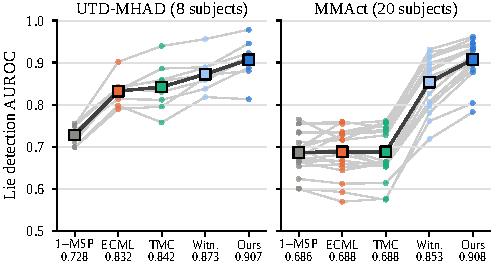
\includegraphics[width=\linewidth]{figs/lie_auroc_per_subject.pdf}
\caption{Per-subject lie detection AUROC on UTD-MHAD (left) and MMAct (right). Each gray line is one test subject; black squares and the numbers under the labels are means over subjects.}
\label{fig:persubject}
\end{figure}

\subsection{Naming the misleading sensor}

On UTD-MHAD the odd-one-out rule was chosen on validation in all 8 folds. It names the lying sensor in 83.1\% [79.0, 87.2] of lie clips (chance 33.3\%): 86.5\% for the inertial unit, 78.8\% for the skeleton and 84.1\% for video (Fig.~\ref{fig:confusion}). TMC and ECML name it in 74.1\% and 67.0\% of clips; the certificate is better for all 8 subjects, by 9.0 [5.0, 13.1] and 16.1 [12.5, 19.7] points. On MMAct, naming between two sensors is at chance level, as expected.

\begin{figure}[t]
\centering
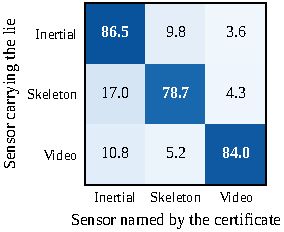
\includegraphics[width=0.62\linewidth]{figs/naming_matrix.pdf}
\caption{Which sensor the certificate names, by the sensor that actually carries the lie (UTD-MHAD, all folds and seeds, \% of each row).}
\label{fig:confusion}
\end{figure}

\subsection{Use, drop or abstain}

\begin{table}[t]
\centering
\caption{Accuracy (\%) after the decision step on UTD-MHAD (mean over 8 test subjects). Rev.\ 2 was designed after rev.\ 1 results.}
\label{tab:policy}
\setlength{\tabcolsep}{4pt}
\begin{tabular}{lccc}
\toprule
System & Normal & Lie & Answer 80\% \\
\midrule
B4 alone & 95.0 & 60.9 & 90.7 \\
Certificate on B4, rev.\ 1 & 93.1 & 72.9 & 91.2 \\
Certificate on B4, rev.\ 2 & 94.9 & 70.5 & 91.9 \\
TMC alone & 94.4 & 74.9 & 89.8 \\
ECML alone, rev.\ 1 & 93.1 & 69.1 & 88.2 \\
\bottomrule
\end{tabular}
\end{table}

Table~\ref{tab:policy} shows the effect of acting on the certificate. With revision 1, accuracy on UTD-MHAD lie clips rises from 60.9\% to 72.9\% (+12.0 points [6.6, 17.4], all 8 subjects), at a cost of 1.9 points on normal clips, of which 18.4\% are dropped. Revision 2 keeps normal accuracy at 94.9\% (6.8\% dropped) and reaches 70.5\% on lie clips. B4 with the certificate still does not reach TMC on lie clips (74.9\%), because B4 is misled more often to begin with. On MMAct only abstention is possible and accuracy on lie clips stays at 29.8\%, below TMC and ECML (42.2\%). The B4 row of the last column uses abstention on $1-$MSP; the TMC and ECML rows use their own revision 1 scores.

\subsection{Certificate on top of TMC}

\begin{table}[t]
\centering
\caption{TMC alone vs.\ the certificate on top of TMC (rev.\ 1 unless marked). Differences: mean [95\% interval], subjects improved.}
\label{tab:ontmc}
\setlength{\tabcolsep}{2.5pt}
\footnotesize
\begin{tabular}{llcccc}
\toprule
 & Metric & TMC & +Cert. & Diff. [95\% CI] & Better \\
\midrule
\multirow{4}{*}{UTD} & Lie AUROC & 0.842 & 0.856 & +0.014 [$-$0.012, 0.040] & 5/8 \\
 & Naming (\%) & 74.1 & 83.1 & +9.0 [5.0, 13.1] & 8/8 \\
 & Lie acc. (\%) & 74.9 & 75.9 & +1.1 [$-$0.5, 2.6] & 4/8 \\
 & Normal acc. (\%) & 94.4 & 93.8 & $-$0.6 [$-$1.7, 0.4] & 0/8 \\
\midrule
\multirow{4}{*}{MMAct} & Lie AUROC & 0.688 & 0.845 & +0.157 [0.142, 0.173] & 20/20 \\
 & Lie acc. (\%) & 42.2 & 42.2 & 0.0 & 0/20 \\
 & Ans. 80\% & 72.5 & 72.0 & $-$0.6 [$-$1.4, 0.2] & 8/20 \\
 & Ans. 80\%, rev. 2 & 74.6 & 77.1 & +2.4 [2.0, 2.9] & 20/20 \\
\bottomrule
\end{tabular}
\end{table}

Table~\ref{tab:ontmc} applies the unchanged certificate to TMC. On MMAct it raises lie detection from 0.688 to 0.845 for every test subject, which shows that the witness signals carry information that TMC's uncertainty does not. Accuracy on lie clips is unchanged because only abstention is available with two sensors; with the revision 2 abstention score, accuracy on the 80\% least suspicious clips rises by 2.4 points for all 20 subjects. On UTD-MHAD the clear gain is naming (83.1\% against 74.1\%, all subjects); the changes in lie detection and lie-clip accuracy are small and their intervals include zero, and normal accuracy is slightly lower. With revision 2 on UTD-MHAD, accuracy on the 80\% least suspicious clips is 93.9\% against 94.5\% for TMC alone.

\section{Discussion and Limitations}

The results support a narrow claim: independent unimodal witnesses detect a misleading sensor better than the confidence of a fused model and better than the uncertainty of TMC and ECML, they can name the sensor when at least three are available, and they add to TMC without retraining it. They do not support a claim that the certificate makes final answers more often correct than TMC. TMC is less often misled by a single sensor, and the certificate's decision step recovers much, but not all, of B4's loss.

The study has further limitations. The lies are constructed by swapping real recordings of the same subject; real faults such as drift, partial dropout or timing errors are not yet tested. UTD-MHAD has 8 subjects, so several differences have wide intervals. Revision 2 of the decision step was designed after seeing revision 1 results; we report both. Naming is not possible on MMAct with two sensors. The witnesses add training and inference cost proportional to the number of sensors.

Future work will add MMAct video as a third sensor so that naming can be tested on a second dataset, evaluate the 247 MMAct clips in which the watch did not record, extend the comparison to further fusion methods and datasets, and study more types of faults.

\section{Conclusion}

Agreement between sensors is not a sufficient basis for trust in multimodal HAR: a single real but wrong stream can mislead a fusion transformer while its confidence stays high. TrustMI-HAR attaches to each prediction a certificate built from unimodal witnesses. Under leave-one-subject-out evaluation on UTD-MHAD and MMAct it detects misleading sensors better than confidence scores, TMC and ECML for every test subject, names the misleading sensor in 83.1\% of UTD-MHAD lie clips, and improves TMC's lie detection on MMAct from 0.688 to 0.845 when placed on top of it.

\begin{thebibliography}{99}

\bibitem{wang2019survey}
J. Wang, Y. Chen, S. Hao, X. Peng, and L. Hu, ``Deep learning for sensor-based activity recognition: A survey,'' \textit{Pattern Recognition Letters}, vol. 119, pp. 3-11, 2019.

\bibitem{chen2015utd}
C. Chen, R. Jafari, and N. Kehtarnavaz, ``UTD-MHAD: A multimodal dataset for human action recognition utilizing a depth camera and a wearable inertial sensor,'' in \textit{Proc. IEEE Int. Conf. Image Processing (ICIP)}, 2015, pp. 168-172.

\bibitem{kong2019mmact}
Q. Kong, Z. Wu, Z. Deng, M. Klinkigt, B. Tong, and T. Murakami, ``MMAct: A large-scale dataset for cross modal human action understanding,'' in \textit{Proc. IEEE/CVF Int. Conf. Computer Vision (ICCV)}, 2019, pp. 8658-8667.

\bibitem{hendrycks2017baseline}
D. Hendrycks and K. Gimpel, ``A baseline for detecting misclassified and out-of-distribution examples in neural networks,'' in \textit{Proc. Int. Conf. Learning Representations (ICLR)}, 2017.

\bibitem{sensoy2018evidential}
M. Sensoy, L. Kaplan, and M. Kandemir, ``Evidential deep learning to quantify classification uncertainty,'' in \textit{Advances in Neural Information Processing Systems (NeurIPS)}, 2018, pp. 3179-3189.

\bibitem{han2021tmc}
Z. Han, C. Zhang, H. Fu, and J. T. Zhou, ``Trusted multi-view classification,'' in \textit{Proc. Int. Conf. Learning Representations (ICLR)}, 2021.

\bibitem{xu2024ecml}
C. Xu, J. Si, Z. Guan, W. Zhao, Y. Wu, and X. Gao, ``Reliable conflictive multi-view learning,'' in \textit{Proc. AAAI Conf. Artificial Intelligence}, vol. 38, no. 14, 2024, pp. 16129-16137.

\bibitem{ma2022missing}
M. Ma, J. Ren, L. Zhao, D. Testuggine, and X. Peng, ``Are multimodal transformers robust to missing modality?'' in \textit{Proc. IEEE/CVF Conf. Computer Vision and Pattern Recognition (CVPR)}, 2022, doi: 10.1109/CVPR52688.2022.01764.

\bibitem{yang2021defending}
K. Yang, W.-Y. Lin, M. Barman, F. Condessa, and Z. Kolter, ``Defending multimodal fusion models against single-source adversaries,'' in \textit{Proc. IEEE/CVF Conf. Computer Vision and Pattern Recognition (CVPR)}, 2021, pp. 3340-3349.

\bibitem{zhang2023qmf}
Q. Zhang, H. Wu, C. Zhang, Q. Hu, H. Fu, J. T. Zhou, and X. Peng, ``Provable dynamic fusion for low-quality multimodal data,'' in \textit{Proc. Int. Conf. Machine Learning (ICML)}, 2023, pp. 41753-41769.

\bibitem{liu2020energy}
W. Liu, X. Wang, J. Owens, and Y. Li, ``Energy-based out-of-distribution detection,'' in \textit{Advances in Neural Information Processing Systems (NeurIPS)}, 2020.

\bibitem{geifman2017selective}
Y. Geifman and R. El-Yaniv, ``Selective classification for deep neural networks,'' in \textit{Advances in Neural Information Processing Systems (NeurIPS)}, 2017, pp. 4878-4887.

\bibitem{lin1991divergence}
J. Lin, ``Divergence measures based on the Shannon entropy,'' \textit{IEEE Trans. Information Theory}, vol. 37, no. 1, pp. 145-151, 1991.

\bibitem{tran2018closer}
D. Tran, H. Wang, L. Torresani, J. Ray, Y. LeCun, and M. Paluri, ``A closer look at spatiotemporal convolutions for action recognition,'' in \textit{Proc. IEEE/CVF Conf. Computer Vision and Pattern Recognition (CVPR)}, 2018, pp. 6450-6459.

\bibitem{kay2017kinetics}
W. Kay et al., ``The Kinetics human action video dataset,'' arXiv:1705.06950, 2017.

\bibitem{vaswani2017attention}
A. Vaswani et al., ``Attention is all you need,'' in \textit{Advances in Neural Information Processing Systems (NeurIPS)}, 2017.

\bibitem{loshchilov2019adamw}
I. Loshchilov and F. Hutter, ``Decoupled weight decay regularization,'' in \textit{Proc. Int. Conf. Learning Representations (ICLR)}, 2019.

\end{thebibliography}

\end{document}
